\documentclass [12pt]{article}


\usepackage{ucs}
\usepackage[utf8x]{inputenc} %Поддержка UTF8
\usepackage{cmap} % Улучшенный поиск русских слов в полученном pdf-файле
\usepackage[english,russian]{babel} %Пакет для поддержки русского и английского языка
\usepackage{graphicx} %Поддержка графиков
\usepackage{float} %Поддержка float-графиков
\usepackage[left=20mm,right=15mm, top=20mm,bottom=20mm,bindingoffset=0cm]{geometry}
\usepackage{mathtools} 
\usepackage{setspace,amsmath}
\usepackage{amsmath,amssymb}
\usepackage{dsfont}
\renewcommand{\baselinestretch}{1.2}
 
\usepackage{color} 
\definecolor{deepblue}{rgb}{0,0,0.5}
\definecolor{deepred}{rgb}{0.6,0,0}
\definecolor{deepgreen}{rgb}{0,0.5,0}

\DeclareFixedFont{\ttb}{T1}{txtt}{bx}{n}{12} % for bold
\DeclareFixedFont{\ttm}{T1}{txtt}{m}{n}{12}  % for normal

\usepackage{listings}
 
\lstset{
	language=Python,
	basicstyle=\ttm,
	otherkeywords={self},             % Add keywords here
	keywordstyle=\ttb\color{deepblue},
	emph={MyClass,__init__},          % Custom highlighting
	emphstyle=\ttb\color{deepred},    % Custom highlighting style
	stringstyle=\color{deepgreen},
	frame=tb,                         % Any extra options here
	showstringspaces=false            % 
}
 
\usepackage{hyperref}
 
\hypersetup{
    bookmarks=true,         % show bookmarks bar?
    unicode=false,          % non-Latin characters in Acrobat’s bookmarks
    pdftoolbar=true,        % show Acrobat’s toolbar?
    pdfmenubar=true,        % show Acrobat’s menu?
    pdffitwindow=false,     % window fit to page when opened
    pdfstartview={FitH},    % fits the width of the page to the window
    pdftitle={My title},    % title
    pdfauthor={Author},     % author
    pdfsubject={Subject},   % subject of the document
    pdfcreator={Creator},   % creator of the document
    pdfproducer={Producer}, % producer of the document
    pdfkeywords={keyword1} {key2} {key3}, % list of keywords
    pdfnewwindow=true,      % links in new PDF window
    colorlinks=true,       % false: boxed links; true: colored links
    linkcolor=black,          % color of internal links (change box color with linkbordercolor)
    citecolor=green,        % color of links to bibliography
    filecolor=magenta,      % color of file links
    urlcolor=cyan           % color of external links
}

\title{}
\date{}
\author{}

\begin{document}
\begin{titlepage}
\thispagestyle{empty}
\begin{center}
Федеральное государственное бюджетное образовательное учреждение высшего профессионального образования \\Московский государственный технический университет имени Н.Э. Баумана

\end{center}
\vfill
\centerline{\large{Лабораторная работа №2}}
\centerline{\large{по курсу <<Численные методы>>}}
\centerline{\large{<<Интерполяция B-сплайнами>>}}
\vfill
\hfill\parbox{5cm} {
           Выполнил:\\
           студент группы ИУ9-62 \hfill \\
           Иванов Георгий\hfill \medskip\\
           Проверила:\\
           Домрачева А.Б.\hfill
       }
\centerline{Москва, 2017}
\clearpage
\end{titlepage}

\textsc{\textbf{Цель:}} 

Анализ метода интерполяции функции, основанный на построении B-сплайна в контрольных точках.

\textsc{\textbf{Постановка задачи:}} 

\textbf{Дано:}  Функция $y_i = \phi(x_i),  i = \overline{1,n}$ задана таблично, исходные данные включают ошибки измерения.

\begin{table}[h]
\begin{center}
\begin{tabular}{|c|c|c|c|c|}
\hline
$x_1$ & $x_2$ & ... & $x_{n-1}$ & $x_n$ \\
\hline
$y_1$ & $y_2$ & ... & $y_{n-1}$ & $y_n$ \\
\hline
\end{tabular}
\end{center}
\end{table}

\textbf{Найти:} Функцию (интерполянту) $f(x)$, совпадающую с значениями $y_i, i = \overline{1,n}$ в контрольных точках $x_i, i = \overline{1,n}$:
$$f(x_i)=y_i$$

\textbf{Тестовый пример:} 

Зададим некоторую функцию $\phi(x)$ таблично:

\begin{table}[h]
\begin{center}
\begin{tabular}{|c|c|c|c|c|c|c|c|c|c|c|}
\hline
0.5 & 0.75 & 1.0 & 1.25 & 1.5 & 1.75 & 2.0 & 2.25 & 2.5 & 2.75\\
\hline
2.78 & 2.95 & 3.13 & 3.31 & 3.c51 & 3.72 & 3.94 & 4.18 & 4.43 & 4.69\\
\hline
\end{tabular}
\end{center}
\end{table}

\begin{table}[h]
\begin{center}
\begin{tabular}{|c|c|c|c|c|c|c|c|c|c|c|}
\hline
3.0 & 3.25 & 3.5 & 3.75 & 4.0 & 4.25 & 4.5 & 4.75 & 5.0 & 5.25 & 5.5 \\
\hline
4.97 & 5.27 & 5.58 & 5.92 & 6.27 & 6.65 & 7.04 & 7.47 & 7.91 & 8.38 & 8.89 \\
\hline
\end{tabular}
\end{center}
\end{table}

\textbf{Теоретические сведения:}

Интерполяция, интерполирование — в вычислительной математике способ нахождения промежуточных значений величины по имеющемуся дискретному набору известных значений.

Основная цель интерполяции — получить быстрый (экономичный) алгоритм вычисления значений $y(x)$ для значений $x$, не содержащихся в таблице данных.
Интерполируюшие функции $f(x)$, как правило строятся в виде линейных комбинаций некоторых элементарных функций:
$$f(x)=\sum_{k=0}^N {c_k\Phi_k(x)}$$
где $\{\Phi_k(x)\}$ — фиксированный линейно независимые функции, $c_0, c_1, \cdots, c_n$ — не определенные пока коэффициенты.

Один из способов интерполирования на всем отрезке $[a, b]$ является интерполирование сплайнами.
Сплайном называется кусочно-полиномиальная функция, определенная на отрезке $[a, b]$ и имеющая на этом отрезке некоторое количество непрерывных производных. Преимущества интерполяции сплайнами по сравнению с обычными методами интерполяции – в сходимости и устойчивости вычислительного процесса.

Рассмотрим один из наиболее распространенных в практике случаев – интерполирование функции кубическим сплайном.

Пусть на отрезке $[a, b]$ задана непрерывная функция $y(x)$. Введем разбиение отрезка:
$$ a = x_0 < x_1 < x_2 < \cdots < x_{n-1} < x_n = b $$ и обозначим $y_i=y(x_i),  i = \overline{1,n}$

Сплайном, соответствующим данной функции узлам интерполяции называется функция $s(x)$, удовлетворяющая следующим условиям:
\begin{enumerate}
\item На каждом отрезке $[x_{i-1};x_{i}],  i = \overline{2,n}$ функция $s(x)$ является кубическим многочленом;
\item Функция $s(x)$, а также ее первая и вторая производные непрерывны на отрезке $[a, b]$;
\item $s(x_i)=y_i,  i = \overline{2,n}$ - условие интерполирования.
\end{enumerate}

Сплайн, определяемый условиями 1 – 3, называется интерполяционным кубическим сплайном.

Также, можно использовать набор кусочно-кубических полиномов для формирования некоторого набора базисных функций, поскольку линейные комбинации этих функций также удовлетворяли бы свойствам непрерывности на границах между смежными интервалами. Тогда чтобы построить кубический сплайн по всему диапазону $[a, b]$, нужно было бы сопоставить сумму базисных функций с табличными значениями $y_i$ в интерполирующих узлах $x_i, i = \overline{1,n}$. 

В-сплайны являются базисными функциями, удовлетворяющими нашим условиям непрерывности. Если интерполяция проводится по области $[a, b]$, то $B_0$ определяется формулой:


\begin{equation*}
B_0(x) =  
\begin{cases}
0 & x \leq x_0 - 2h \\
\frac{1}{6}(2h + (x - x_0))^3 & x_0-2h \leq x \leq x_0 -h \\
\frac{2h^3}{3}-\frac{1}{2}(x-x_0)^2(2h + (x - x_0)) & x_0-h \leq x \leq x_0 \\
\frac{2h^3}{3}-\frac{1}{2}(x-x_0)^2(2h - (x - x_0)) & x_0 \leq x \leq x_0+h \\
\frac{1}{6}(2h - (x - x_0))^3 & x_0+h \leq x \leq x_0 +2h \\
0 & x \geq x_0 + 2h \\
\end{cases}
\end{equation*}
где $h=x_{k+1}-x_{k}=\frac{x_n-x_0}{N}$ - длина интервала между интерполирующими узлами. Заметим, что $B_0$ имеет ненулевые значения над 4 интервалами.

\begin{figure}[h]
\begin{center}
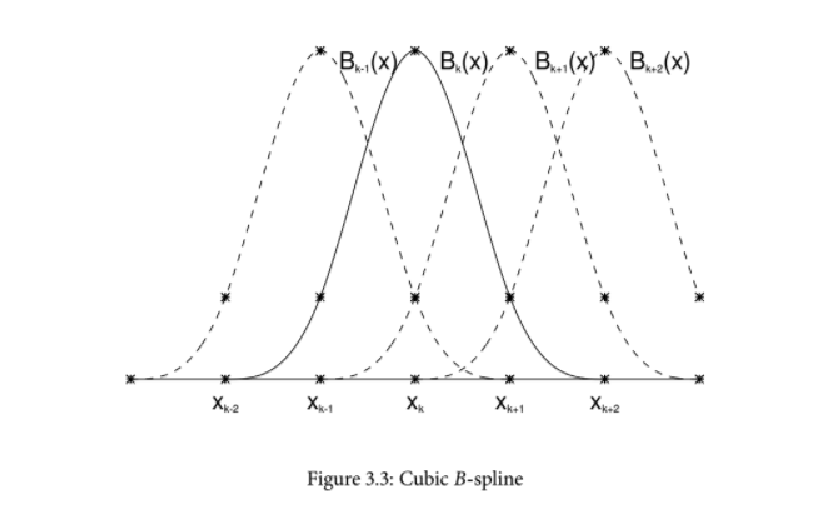
\includegraphics[scale=.9]{2.eps}\\
\textit{Рисунок 1. Кубические базисные B-сплайны}
\end{center}
\end{figure}

Определим $B_k(x)=B_0(x-kh+x_0)$, так как функции $B_0$ сдвинуты вправо на k узлов. Также заметим, что $B_{k-1}$,$B_{k}$,$B_{k+1}$,$B_{k+2}$ - ненулевые на интервале $[x_{k};x_{k+1}]$.

Кубический сплайн $s_{3}(x)$, определенный на интервале $[x_0;x_n]$, расписывается в виде линейной комбинации $B_k$:
$$s_{3}(x) = \sum_{k=-1}^{N+1} a_kB_k(x) $$
Суммирование начинается с $-1$, так как $B_{-1}$ - ненулевая базисная функция на интервале $[x_0;x_1]$ и заканчивается на $N+1$, так как $B_{N+1}$ - ненулевая базисная функция на интервале $[x_{N-1};x_N]$.

Для проверки третьего условия интерполяционного кубического сплайна возьмём условие $s_3^{''}(x_0)=s_3^{''}(x_N)=0$ (кривизна на границах равна 0).
Распишем его. 

\begin{equation*}
\begin{cases}
B_{k}(x_k) = &B_{0}(x_0) = \frac{2h^3}{3}\\
B_{k-1}(x_k) = & B_{0}(x_0+h) = \frac{h^3}{6} \\
B_{k+1}(x_k) = & B_{0}(x_0-h) = \frac{h^3}{6} \\
B_{k+2}(x_k) = & B_{0}(x_0-2h)  = 0 \\
\end{cases}
\end{equation*}

Получим формулу для вычисления коэффициентов сплайна $a_k$:
$$a_{k-1}+4a_{k}+a_{k+1}=\frac{6}{h^3} y_k$$ для $k=\overline{0..N}$
Вычисляя вторую производную от $B_0$ получим матричное уравнение для вычисления коэффициентов сплайна $a_k$:
$$\left(\begin{array}{cccccc} 
1 & 0 & 0 & ... & ... &  0 \\
1 & 4 & 1 & ... & ... &  0 \\
0 & 1 & 4 & 1 & ... &  0 \\
\vdots & ... & \ddots & \ddots & \ddots &  \vdots \\
0 & ... & ... & 1 & 4 & 1 \\
0 & ... & ... & ... & 0 & 1\\
\end{array}\right) 
\left(\begin{array}{c} 
a_0 \\
a_1 \\
a_2 \\
\vdots \\
a_{N-1} \\
a_{N} \end{array}\right) =
\frac{1}{h^3} \left(\begin{array}{c} 
y_0 \\
6y_1 \\
6y_2 \\
\vdots \\
6y_{N-1} \\
6y_{N} \end{array}\right)   $$
Данные коэффициенты будем искать с помощью метода прогонки.

\textsc{\textbf{Практическая реализация:}}
Листинг 1. Интерполяция B-сплайнами
\begin{lstlisting}[language=python]
#!python
# -*- coding: utf-8 -*-

def tridiagonalMatrixAlgorithm(d,c,a,b):
    alpha = [-c[0]/d[0]]
    beta = [b[0]/d[0]]
    n = len(b)

    for i in range(1,n):
        alpha.append(-c[i]/(d[i]+alpha[i-1]*a[i]))
        beta.append((b[i]-a[i]*beta[i-1])/(d[i]+alpha[i-1]*a[i]))

    x = [0 for _ in range(n+2)]
    x[n+1]=beta[n-1]
    n -= 1
    for i in range(n,0,-1):
        x[i]=x[i+1]*alpha[i-1]+beta[i-1]
    x[0] = 2*x[1]-x[2]
    x[n+2]=2*x[n+1]-x[n]
    return x

def spline(len,ys,h):
    size = len
    n = size-1
    d = [1]
    c = [0]
    a = [0]
    b = [ys[0]]

    for i in range(1,n):
        d.append(4)
        c.append(1)
        a.append(1)
        b.append(6*ys[i])

    d.append(1)
    c.append(0)
    a.append(0)
    b.append(0)

    for i in range(0,n):
        b[i] /= (h*h*h)

    e = tridiagonalMatrixAlgorithm(d,c,a,b)

    return e

def baseX(k,xs,x,h,kh):
    x0 = xs[0]
    if k == 0:
        if x0 + 2 * h <= x: 
            return 0
        if x0 + h <= x and x < x0 + 2 * h: 
	    return (2 * h + x0 - kh - (x - kh)) ** 3 / 6
        if x0 <= x and x <= x0+h: 
 	    return 2*h**3/3 - ((x-x0) ** 2 * (2*h + x0 - kh - (x - kh))) / 2
        if x0 - h <= x and x < x0: 
            return 2 * h ** 3 / 3 - ((x - x0) ** 2 *\
		     (2 * h - x0 + kh + (x - kh))) / 2
        if x0 - 2 * h <= x and x < x0 - h:
            return (2 * h - x0 + kh + (x - kh)) ** 3 / 6
        if x <= x0 - 2 * h: 
            return 0
    else:
        return baseX(0,xs,x-k*h,h,-k*h)

def countSpline(spl,val,n,xs,h):
    i = 0
    for i in range(0,n+2):
        if xs[i] <= val and val <= xs[i+1]:
            break

    if n+2 == i:
        i-=1

    return spl[i+0] * baseX(i-1,xs,val,h,0) +\
	      spl[i+1] * baseX(i,  xs,val,h,0) +\
	      spl[i+2] * baseX(i+1,xs,val,h,0) +\
	      spl[i+3] * baseX(i+2,xs,val,h,0)


if __name__ == "__main__":

    xs = [0.5, 1.0, 1.5, 2.0, 2.5, 3.0, 3.5, 4.0, 4.5, 5.0, 5.5]
    ys = [2.78, 3.13, 3.51, 3.94, 4.43, 4.97, 5.58, 6.27, 7.04, 7.91, 8.89]

    xsNew = [0.50, 0.75, 1.00, 1.25, 1.50, 1.75, 2.00, 2.25, 2.50, 2.75, 
         3.00, 3.25, 3.50, 3.75, 4.00, 4.25, 4.50, 4.75, 5.00, 5.25, 5.50]
    ysNew = [2.78, 2.95, 3.13, 3.31, 3.51, 3.72, 3.94, 4.18, 4.43, 4.69,
         4.97, 5.27, 5.58, 5.92, 6.27, 6.65, 7.04, 7.47, 7.91, 8.38, 8.89]
    N = 10 
    h = 0.5
    print(str)
    spl = spline(N+2,ys,h)
    for i in range(0,2*N+1):
        val = xsNew[i]
        bsVal = countSpline(spl,val,N,xs,h)
        print("x=%f|f(x)=%f ... spl(x)=%f" %(val,ysNew[i],bsVal))
\end{lstlisting}
\textbf{Результаты:}

Для тестирования полученной программы была задана табличная функция:

\begin{table}[h]
\begin{center}
\begin{tabular}{|c|c|c|c|c|c|c|c|c|c|c|}
\hline
0.5 & 0.75 & 1.0 & 1.25 & 1.5 & 1.75 & 2.0 & 2.25 & 2.5 & 2.75\\
\hline
2.78 & 2.95 & 3.13 & 3.31 & 3.c51 & 3.72 & 3.94 & 4.18 & 4.43 & 4.69\\
\hline
\end{tabular}
\end{center}
\end{table}

\begin{table}[h]
\begin{center}
\begin{tabular}{|c|c|c|c|c|c|c|c|c|c|c|}
\hline
3.0 & 3.25 & 3.5 & 3.75 & 4.0 & 4.25 & 4.5 & 4.75 & 5.0 & 5.25 & 5.5 \\
\hline
4.97 & 5.27 & 5.58 & 5.92 & 6.27 & 6.65 & 7.04 & 7.47 & 7.91 & 8.38 & 8.89 \\
\hline
\end{tabular}
\end{center}
\end{table}

В результате работы программы (Листинг 1) получаем значения:

\begin{center}
\begin{tabular}{ |c|c|c|c| }
  \hline
 Значение $x_{n}$ & Значение $y_{n}$ & Значение сплайна $s^{3}(x_n)$ & Разница значений  $s^{3}(x_n)-y_{n}$ \\ \hline
 0.5 & 2.78 & 2.7799999999999994 & -4.440892098500626e-16\\ \hline
 0.75 & 2.95 & 2.952961581335141 & 0.002961581335140906\\ \hline
 1.0 & 3.13 & 3.13 & 0.0\\ \hline
 1.25 & 3.31 & 3.3148652559945737 & 0.004865255994573658\\ \hline
 1.5 & 3.51 & 3.51 & 0.0\\ \hline
 1.75 & 3.72 & 3.7175773946865607 & -0.0024226053134395187\\ \hline
 2.0 & 3.94 & 3.94 & 0.0\\ \hline
 2.25 & 4.18 & 4.178575165259181 & -0.0014248347408187811\\ \hline
 2.5 & 4.43 & 4.43 & 0.0\\ \hline
 2.75 & 4.69 & 4.691871944276711 & 0.0018719442767105576\\ \hline
 3.0 & 4.97 & 4.97 & 0.0\\ \hline
 3.25 & 5.27 & 5.268937057633973 & -0.0010629423660262205\\ \hline
 3.5 & 5.58 & 5.58 & 0.0\\ \hline
 3.75 & 5.92 & 5.901129825187394 & -0.01887017481260589\\ \hline
 4.0 & 6.27 & 6.27 & 0.0\\ \hline
 4.25 & 6.65 & 6.69654364161645 & 0.04654364161644953\\ \hline
 4.5 & 7.04 & 7.039999999999999 & -8.881784197001252e-16\\ \hline
 4.75 & 7.47 & 7.265195608346805 & -0.20480439165319453\\ \hline
 5.0 & 7.91 & 7.909999999999998 & -1.7763568394002505e-15\\ \hline
 5.25 & 8.38 & 9.118923924996324 & 0.7389239249963229\\ \hline
 5.5 & 8.89 & 8.889999999999999 & -1.7763568394002505e-15\\ \hline
\end{tabular}
\end{center}

\textbf{Выводы:}

В ходе выполнения лабораторной работы был рассмотрен метод интерполяции функции, основанный на построении B-сплайна в контрольных точках, так же для метода была написана реализация на языке программирования Python.

Анализируя результаты полученной программы, можно заметить то, что метод интерполяции функции, основанный на построении B-сплайна в контрольных точках, имеет высокую точность вследствие низкой погрешности. Повышая степень кусочно-интерполяционного многочлена, можно добиться еще лучших результатов аппроксимации функции.

\end{document}

